\chapter{Разработка и создание испытательного стенда для измерения реактивных моментов}\label{ch:ch3}

В предыдущих главах были рассмотрены причины возникновения реактивных моментов при повороте оси визирования оптической системы КА. Математическое моделирование и экспериментальная отработка в космосе показали, что полностью учесть все факторы только расчётными методами невозможно. На практике проявляются дополнительные эффекты: люфты и неточности сборки редукторов, упругие деформации узлов крепления, дисбаланс маховиков, неравномерность распределения массы зеркал. Эти факторы приводят к появлению остаточных моментов и резонансных частот, которые трудно заранее оценить аналитически.

Таким образом, расчётных методов недостаточно для полной оценки динамики формирования реактивных моментов. Практика создания и эксплуатации космических оптико-механических систем показывает, что обязательным этапом юстировки аппаратуры является проведение наземных экспериментальных исследований, позволяющих:

\begin{itemize}
	\item проверить адекватность математических моделей;
	\item уточнить значения моментов инерции подвижных узлов;
	\item определить величины остаточных моментов, не поддающихся точному расчёту;
	\item разработать методы балансировки и оптимизации алгоритмов управления приводами.
\end{itemize}
	
Для решения этих задач необходим специализированный измерительный комплекс. В качестве такого комплекса был разработан испытательный стенд, позволяющий рассматривать исследуемую оптическую систему как колебательное звено, откликающееся на приложенный реактивный момент. В результате анализа угловых колебаний рамы стенда с закреплённой аппаратурой удаётся получить количественную оценку некомпенсированных реактивных моментов.

\section{Теоретическая модель стенда}

Разработанный стенд для измерения остаточных реактивных моментов основан на принципе представления исследуемой оптико-механической системы в виде колебательного звена. Подобная постановка позволяет использовать методы динамики твёрдого тела и теории малых колебаний для регистрации и анализа реактивных воздействий.

Динамика стенда описывается уравнением движения:

\begin{equation}
	\label{eq:stadeq}
	J\cdot \frac{d^2\varphi}{dt^2}+b \cdot \frac{d\varphi}{dt}+ c \cdot \varphi = M(t)
\end{equation}

где \(J\) --- момент инерции рамы вместе с установленной оптической системой, \(\varphi\) --- угол поворота рамы относительно равновесного положения, \(b\) --- коэффициент затухания, \(с\) --- коэффициент крутильной жёсткости, \(M(t)\) --- реактивный момент.

В удобной для анализа форме уравнения записывается как:

\begin{equation}
	\label{eq:standeq2}
	\ddot{\varphi}(t) + 2\,\xi\,\omega_0\,\dot{\varphi}(t) + \omega_0^{2}\,\varphi(t)
	= \frac{M(t)}{J}
\end{equation}

где \(\omega_0\) --- собственная частота колебательного звена, \(\xi\) --- коэффициент затухания.

ЛАЧХ колебательного звена показана на рисунке ~\cref{fig:afc}.

\begin{figure}[!h] 
	\centerfloat{
		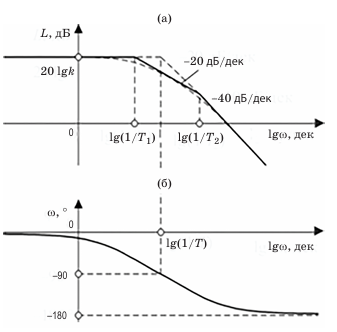
\includegraphics[scale=0.8]{afc} 
	}
	\caption{Логарифмическая амплитудная -а) и логарифмическая фазовая -б) частотные характеристики колебательного звена}
	\label{fig:afc} 
\end{figure}

Для корректного воспроизведения динамики необходимо, чтобы собственная частота маятника была смещена относительно диапазона характерных частот воздействия. В данном случае стенд спроектирован таким образом, что возмущающее воздействие проявляется в послерезонансной области. В этом случае колебательное звено работает как механический фильтр низких частот, подавляющий высокочастотные вибрации основания и внешние помехи, при этом сохраняется информативность основной составляющей измеряемого момента.

Моделирование стенда показало, что при увеличении декремента затухания выше $\xi=0,1$ форма выходного сигнала сильно искажается: снижается амплитуда и появляется фазовый сдвиг относительно входного воздействия (рисунок ~\cref{fig:decrement}). Поэтому при проектировании подвеса использовались материалы и схемы крепления, обеспечивающие малый уровень диссипативных потерь и гарантирующие $\xi \leq 0,1$

\begin{figure}[!h]
	\centering
	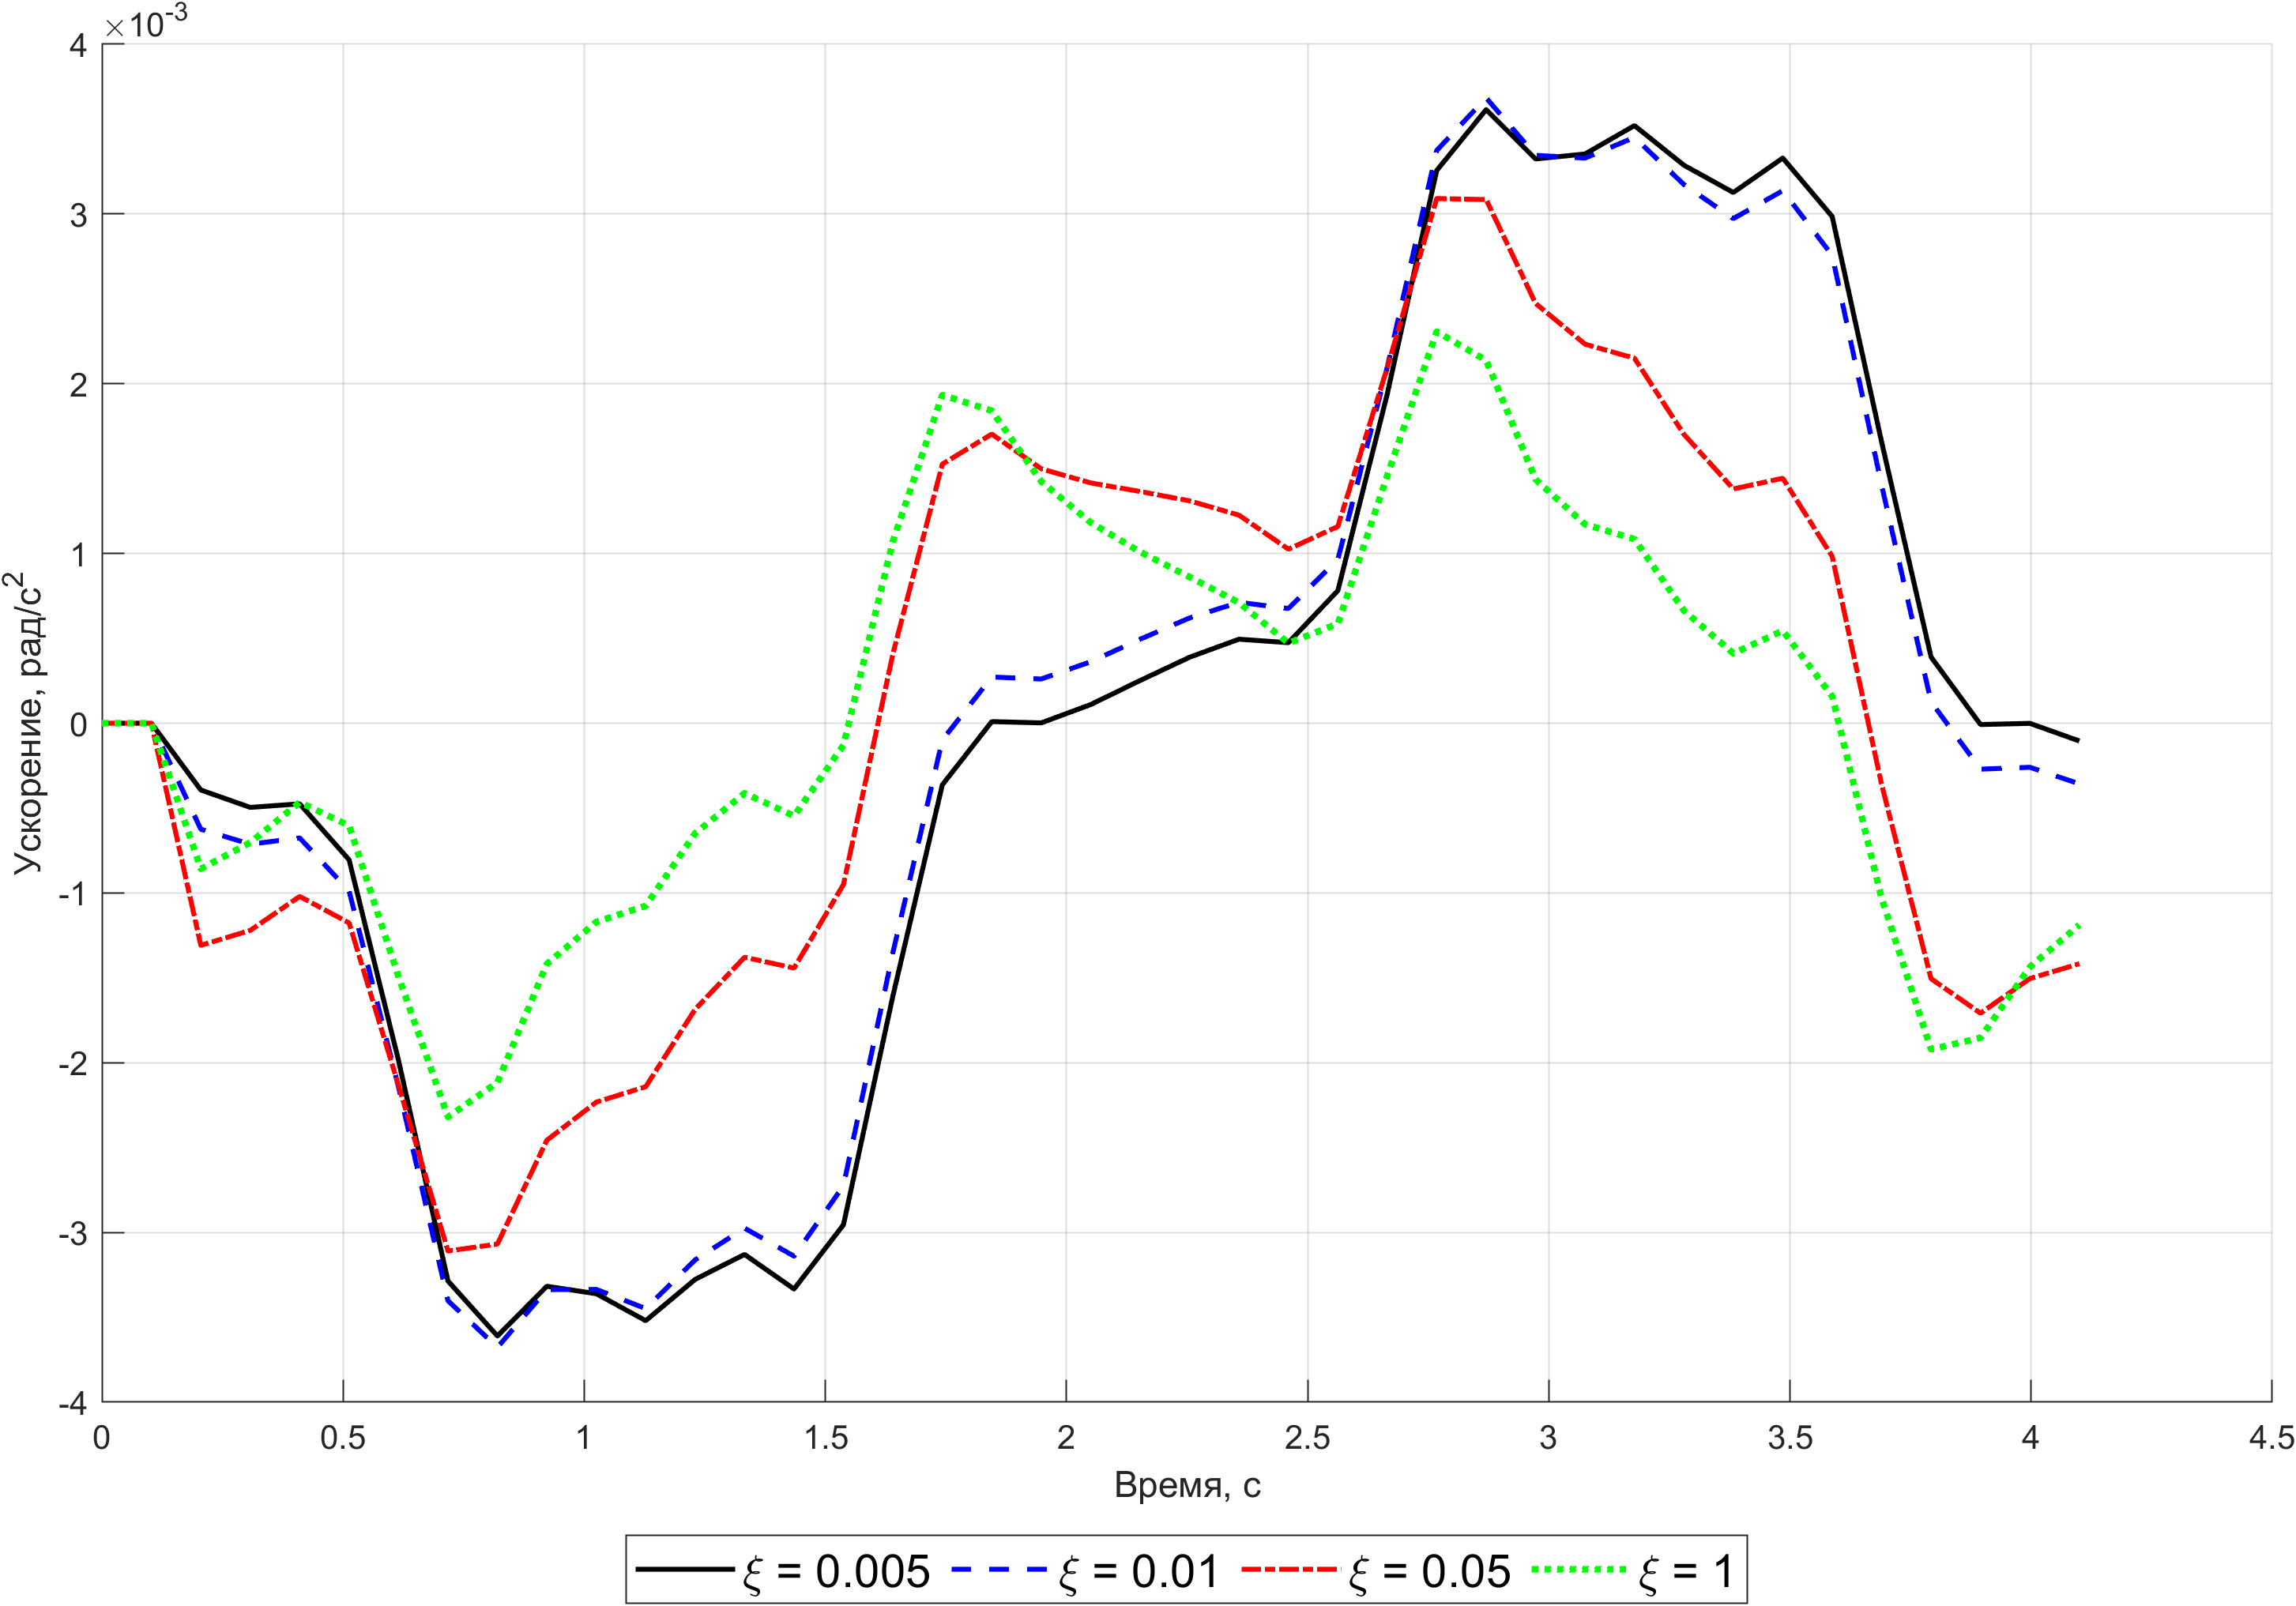
\includegraphics[scale=0.7]{matlab/decrement.png}
	\caption{Ускорение рамы с различными декрементами затухания}
	\label{fig:decrement}
\end{figure}

Таким образом, выбор параметра узла подвеса позволяет:

\begin{itemize}
	\item сместить собственную частоту колебаний стенда в область, лежащую ниже характерных частот рабочего воздействия;
	\item сохранить линейность отклика и минимизировать фазовые искажения;
	\item обеспечить режим работы стенда как фильтра, выделяющего динамику реактивного момента и подавляющего паразитные колебания.
\end{itemize}

\section{Конструктивное устройство стенда}

Измерительный стенд выполнен в виде подвесной системы, обеспечивающей исследуемой ОМС одну степень свободы. Подвижная часть состоит из рамы, подвешенной на двух струнах и способной поворачиваться вокруг вертикальной оси. Внутри рамы установлен жёсткий каркас с основанием для крепления ОМС. Конструкция предусматривает возможность поворота каркаса вокруг горизонтальной оси, что позволяет фиксировать ОМС в двух положениях — с осью $OY$ или $OZ$, совмещённой с направлением струн. Точная балансировка осуществляется с помощью грузов, устанавливаемых на пальцы каркаса.

Настройка стенда проводится таким образом, чтобы центр карданова подвеса совпадал с центром масс каркаса и находился на линии подвесных струн. Для выставления основания в горизонтальное положение используются регулируемые домкраты.

Узел подвеса включает штабелёр, раму на проволочном подвесе, кантователь для ориентации ОМС и балансировочные грузы. При подъёме рамы штабелёром подвес разарретируется и получает возможность свободного вращения на угол ±5° вокруг вертикальной оси. При опускании рама фиксируется ловителями и полностью исключает перемещения относительно основания.

ОМС монтируется на посадочное место кантователя. Поворот кантователя вокруг горизонтальной оси позволяет выбрать направление оси поворота, совпадающей с вертикальной осью стенда. В процессе разворота ОМС возникает реактивный момент, вызывающий вращение рамы вокруг вертикальной оси. Угловое движение регистрируется волоконно-оптическим гироскопом, установленным на подвесной раме. Дополнительно в состав установки включён тестовый маховик с известным моментом инерции, используемый для формирования контролируемого возмущающего момента. Совместное применение гироскопа и маховика обеспечивает как регистрацию угловых колебаний, так и калибровку чувствительности системы.

Установку настраивают таким образом, чтобы центр карданакарданова подвеса и центр масс каркаса оказались на линии струн.

Общий вид установки приведён на рисунке ~\cref{fig:yoiom}.
 
\begin{figure}[!h] 
	\centerfloat{
		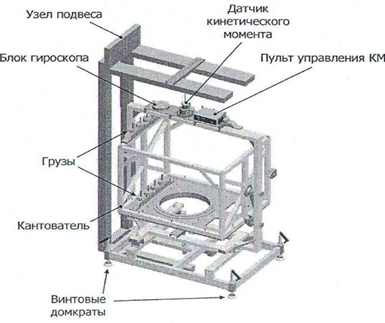
\includegraphics[scale=1.2]{yoim-cxem} 
	}
	\caption{Стенд измерения реактивного момента}
	\label{fig:yoiom} 
\end{figure}

В узел подвеса входит штабелёр , рама на проволочном подвесе, кантователь, установленный в раме, и балансировочные грузы, закреплённые на кантователе. Подъём рамы с помощью штабелёра вверх позволяет разарретировать раму с кантователем; при этом возникает возможность разворота рамы на угол ±5° вокруг вертикальной оси. При опускании рамы с кантователем рама садится на ловители и не имеет свободы перемещения относительно основания устройства.

ОМС устанавливается на посадочное место кантователя, входящего в  узел подвеса стенда. Путём разворота кантователя, вокруг горизонтальной оси выбирается и фиксируется ось поворота ОМС. Ось перенацеливания совпадает с вертикальной осью. 
В момент поворота ОМС возникает некомпенсированный момент вокруг вертикальной оси на подвижную часть устройства, вследствие чего рама узла подвеса стенда вместе с ОМС, установленной в кантователь, начинает вращаться вокруг вертикальной оси. Волоконно-оптический гироскоп регистрирует наличие угловой скорости подвижной части. Дополнительно в состав установки включён тестовый маховик с известным моментом инерции, используемый для формирования контролируемого возмущающего момента.

\section{Методика измерения реактивного момента}

\subsection{Принцип метода измерений}

Методика предназначена для измерения некомпенсированного реактивного момента, возникающего при перемещении подвижных частей ОМС. Диапазон измерений охватывает значения от $10^{-3}$ до $1 \,\text{Н}\cdot\text{м}$.

Применяемый метод относится к категории косвенных. Измерение некомпенсированного момента выполняется через регистрацию скорости колебаний подвесной системы, вызванных реактивным воздействием. Регистрация осуществляется волоконно-оптическим гироскопом, установленным на подвижной раме. Для формирования эталонного воздействия используется тестовый маховик с заранее известным моментом инерции, установленный на отдельном приводе.

Суть метода заключается в сравнении ускорений колебаний подвеса, вызванных реактивным моментом оптико-механической системы, сравнивается с ускорением, возникающим при воздействии тестового маховика. Поскольку момент инерции подвеса в обоих случаях одинаковый, ускорение однозначно определяет величину приложенного момента. 



\subsection{Подготовка к проведению измерений}

Перед началом экспериментов исследуемая оптико-механическая система устанавливается в изделиедержатель стенда и фиксируется на фланце металлического куба. Далее выполняется юстировка подвесной системы. Для этой цели используется регулируемый зацеп, позволяющий смещать точку крепления струны в горизонтальной плоскости. Совмещение оси подвеса с центром масс подвижной части проводится по показаниям пузырькового уровня. После установки и юстировки производится подключение средств измерений и вспомогательного оборудования (см. Таблицу ~\cref{tab:measures}). Включение аппаратуры выполняется заблаговременно, не менее чем за 30 минут до начала измерений, что необходимо для термостабилизации гироскопа и электронной части измерительной системы.

В обязательном порядке проверяется работоспособность волоконно-оптического гироскопа. Для этого прибор фиксируется на неподвижном основании и регистрирует проекцию угловой скорости вращения Земли. Измеренное значение сравнивается с расчётным, определяемым по географической широте места проведения эксперимента. Допустимое расхождение не должно превышать 0,3 \%, что подтверждает пригодность гироскопа к дальнейшему использованию. %todo subsubsection

%todo график гироскопа

Гироскоп устанавливают в неподвижное положение на виброизолированном стенде. Выходной сигнал~$\omega_g(t)$ снимают в течение двух часов с частотой $f_s = \SI{100}{\hertz}$
Результаты приведены на рисунке~\cref{fig:Earth}.

\begin{figure}[ht]
	\centerfloat{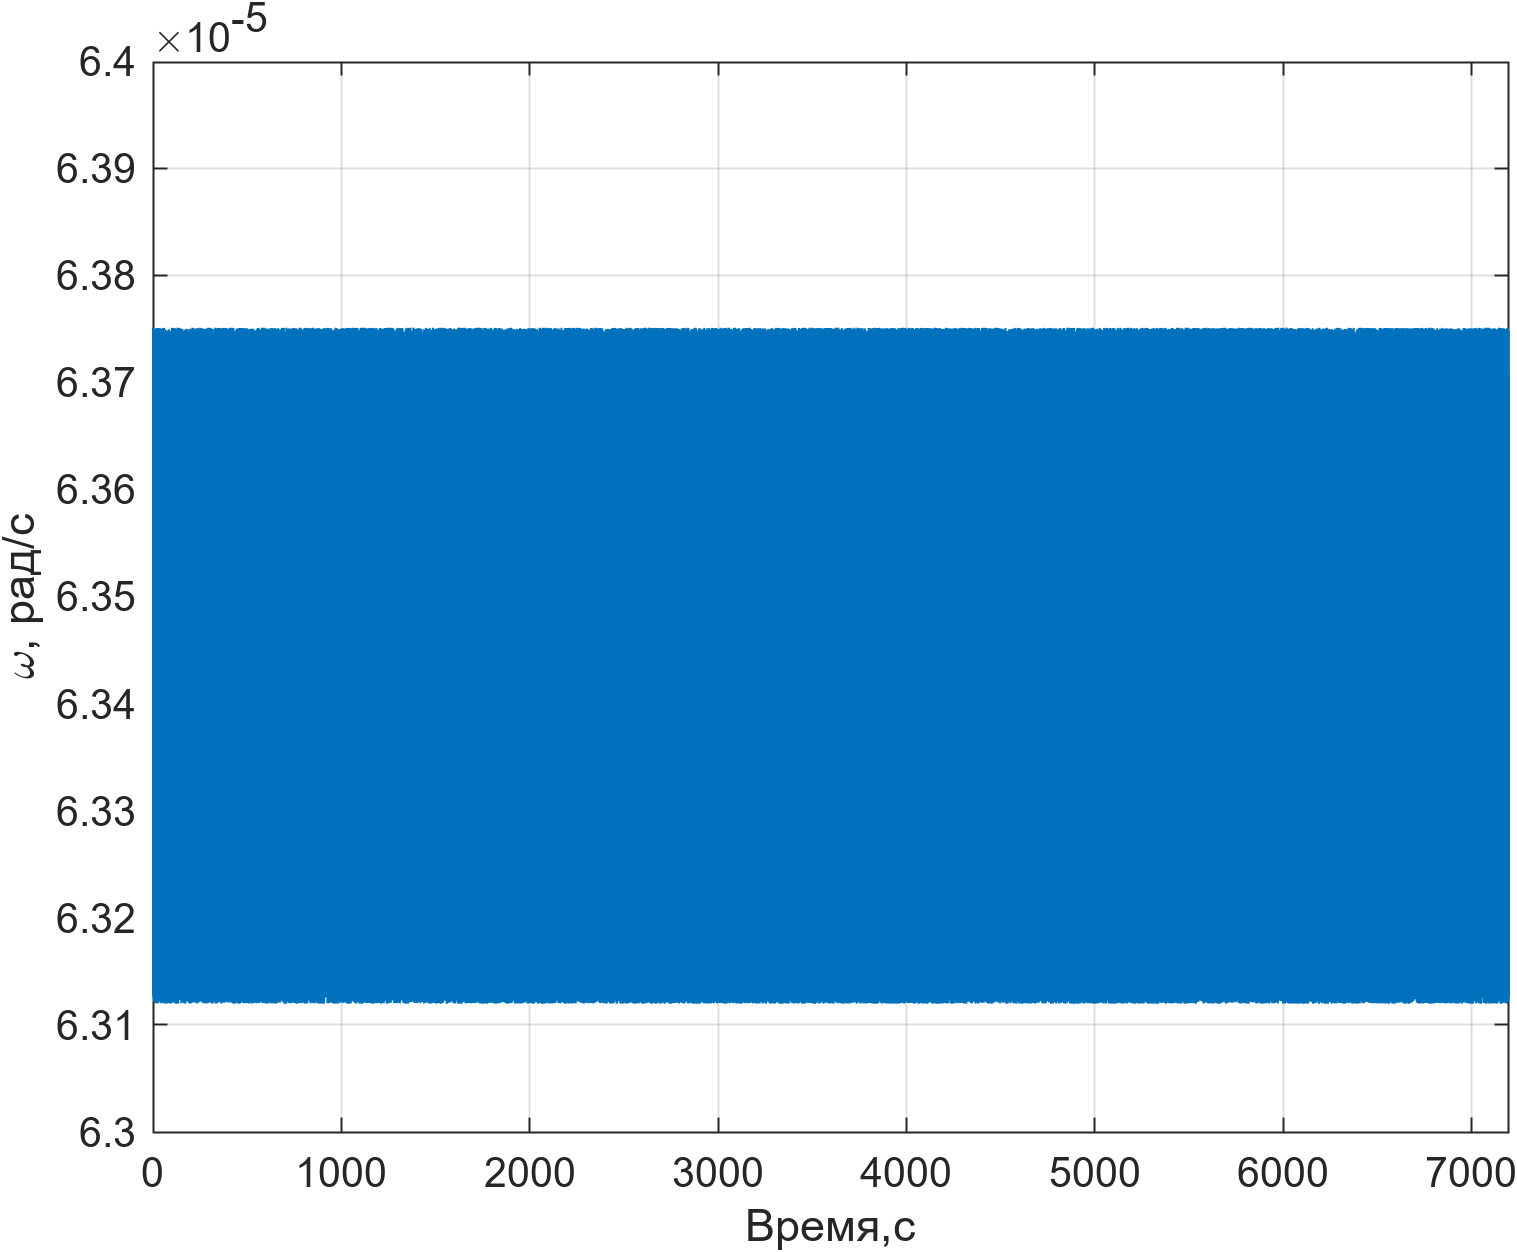
\includegraphics[scale=0.8]{matlab/gyroEarth.png}}
	\caption{Измерение проекции угловой скорости вращения Земли}
	\label{fig:Earth}
\end{figure}

Математическое ожидание сигнала гироскопа:
\begin{equation}
	\bar{\omega}
	= \frac{1}{N}\sum_{i=1}^{N}\omega_g(t_i)
	\label{eq:mean}
\end{equation}

По расчётам среднее значение составляет 
$
\bar{\omega} = \SI{6,34 e-5}{\text{рад/c}}
$

Угловая скорость вращения Земли
$\Omega_E = 2\pi/T_{\text{сут}}\approx \SI{7,292 e-5}{\text{рад/с}}.
$
На широте города Санкт-Петербург $\phi_{\mathrm{e}} = 59^\circ57'$ получаем проекцию на вертикальную ось гироскопа:
\[
\omega_e
= \Omega_E\sin\phi_{\text{e}}
\approx 7.292\cdot10^{-5}\sin(59^\circ57')
\approx 6.32\times10^{-5}\text{рад/с}\\
\]

Смещение нуля:
\begin{equation}
	\epsilon
	= \bar{\omega} - \omega_e = \SI{3,16 e-7}{\text{рад/c}}
	\label{eq:omega_correct}
\end{equation}

Оценка шумовой составляющей. Дисперсия определяется по формуле:
\begin{equation}
	\sigma^2=\frac{1}{N-1}\sum_{i=1}^N(\omega_i-\bar{\omega})^2
	\label{eq:disperssion}
\end{equation}

Дисперсия составляет: $\sigma^2=\SI{3,15 e-7}{\text{рад/c}} \approx \SI{0,006}{^\circ /c}$

Итоговая погрешность измерения скорости определяется по формуле:
\begin{equation}
	\Delta_{\omega}=\sqrt{\epsilon^2+\sigma^2}=\SI{3,645 e-7}{\text{рад/c}}
	\label{eq:rmse}
\end{equation}

Для измерений нам требуется ускорение, а ускорение определяется как:
\begin{equation}
	\alpha =\frac{\omega_i-\omega_{i-1}}{\Delta t}
	\label{eq:acc}
\end{equation}
Ошибка измерения составляет:
\begin{equation}
	\Delta_\alpha = \frac{\sqrt{2}\sigma}{\Delta t} = \SI{2,57 e-5}{\text{рад}/c^2}
	\label{eq:rmse_a}
\end{equation}







Непосредственно перед измерениями контролируются условия окружающей среды. Температура воздуха в помещении должна находиться в пределах 15–35 °С, относительная влажность — 45–80 \%, атмосферное давление — 84–107 кПа. Контроль осуществляется с помощью барометра-анероида и психрометра. Соблюдение указанных параметров исключает влияние климатических факторов на точность эксперимента. Необходимые средства измерений представлены в таблице ~\cref{tab:measures}

\begingroup
\small
\captionsetup[table]{skip=7pt}

\begin{longtable}{|>{\raggedright\arraybackslash}p{5cm}|
		>{\raggedright\arraybackslash}p{8cm}|
		>{\raggedright\arraybackslash}p{3cm}|}
	\caption{Средства измерений}\label{tab:measures}\\[-0.45\onelineskip]
	\hline
	\textbf{Наименование} & \textbf{\raggedright Метрологические и технические характеристики} & \textbf{\raggedright Измеряемая величина} \\
	\hline
	\endfirsthead
	
	\caption*{Продолжение таблицы~\thetable}\\[-0.45\onelineskip]
	\hline
	\textbf{Наименование} & \textbf{Метрологические и технические характеристики} & \textbf{Измеряемая величина} \\
	\hline
	\endhead
	
	\hline
	\endfoot
	
	\hline
	\endlastfoot
	
	Барометр-анероид метрологический БАММ-1 \newline(№ ФИФ ОЕИ 10069-11)
	& Диапазон измерений давлений от 80 до \SI{106}{\kilo\pascal} (от 600 до \si{800\text{~мм рт. ст.}})
	Пределы допускаемой основной погрешности после введения поправок из паспорта $\pm\SI{0,2}{\kilo\pascal}$ ($\pm \si{1,5\text{~мм рт. ст.}}$)
	& Атмосферное давление            \\ \hline
	
	Психрометр аспирационный МВ-4-2М \newline(№ ФИФ ОЕИ 10069-11)
	& Диапазон измерения температуры: \newline от минус 25 до \SI{50}{\degreeCelsius};\newline Пределы допускаемой погрешности измерений температуры не более $\pm \SI{0,1}{\degreeCelsius}$; \newline Диапазон измерений относительной влажности: от 10 до 100 \%.
	& Относительная влажность воздуха, температура \\ \hline
	
	Преобразователь угловых перемещений ЛИР-ДА190К \newline(№ ФИФ ОЕИ 80050-20)
	& Диапазон измерений от 0 до \SI{360}{\degree}; \newline Пределы допускаемой абсолютной погрешности измерений: $\pm10 "$.
	& Угол разворота \\ \hline
	
	Штангенциркуль ШЦЦ-I-125-0,01
	\newline (№ ФИФ ОЕИ 81768-21)
	& Диапазон измерения от 0 до 125 мм; Шаг дискретности цифрового отсчётного устройства $\SI{0,01}{\milli\meter}$; Пределы допускаемой абсолютной погрешности $\SI{\pm0,03}{\milli\meter}$.
	& Геометрические размеры маховика\\ \hline
	
	Осциллограф TDS1012B \newline (№ ФИФ ОЕИ 32618-06) 
	& Диапазон установки коэффициентов отклонения 10 $\si{\text{мВ/дел - }5\text{В/дел.}}$
	\newline Погрешность установки коэффициентов отклонения: $\pm3$ \%.
	\newline Диапазон коэффициента развёртки $\si{5\text{нс/дел}-50\text{с/дел.}}$
	\newline Пределы допускаемой абсолютной погрешности измерения временных интервалов: $\pm(K_p/250+50 \cdot10^{-6}\cdot T + 0,6 )$, где \(K_p\) "---коэффициент развёртки, \(T\) "---измеряемый временной интервал, с.
	&Временные  интервалы\\ \hline
	
	
	Весы электронные EK-12Ki
	\newline (ФИФ ОЕИ 25312-03)
	& Наибольший предел взвешиваний $\SI{12}{\kilogram}$; наименьший предел взвешивания $\SI{20}{\gram}$; предел допускаемой погрешности $\SI{\pm3}{\gram}$.
	& Масса маховика.\\ \hline
	
	Волоконно-
	\newline оптический гироскоп ОИУС-1000
	&Диапазон измеряемой угловой скорости: $\SI{\pm550}{\degree\per\second}$.
	\newline Случайная составляющая нулевого сигнала при постоянной температуре при осреднении 100 секунд не более $\SI{0,01}{\degree\per\hour}$.
	\newline Случайная составляющая нулевого сигнала в диапазоне рабочих температур при скорости изменения температуры $\SI{0,4}{\degreeCelsius\per\min}$ не более $\SI{0,1}{\degree\per\hour}$.
	\newline Погрешность измерения угловой скорости не более $0,01$ \%.
	&Угловая скорость	\\ \hline
	
\end{longtable}
\normalsize
\endgroup








\subsection{Определение тестового момента}

Для задания эталонного воздействия на подвес используется тестовый маховик, установленный на отдельном приводе. 

При подаче напряжения на двигатель, маховик начинает вращение по заданному закону изменения угловой скорости. Управляющая система обеспечивает трапецеидальный профиль разгона, что позволяет выделить участок равномерного ускорения. Профиль разгона показан на рисунке ~\cref{fig:flyweel_speed}.

\begin{figure}[!h] 
	\centerfloat{
		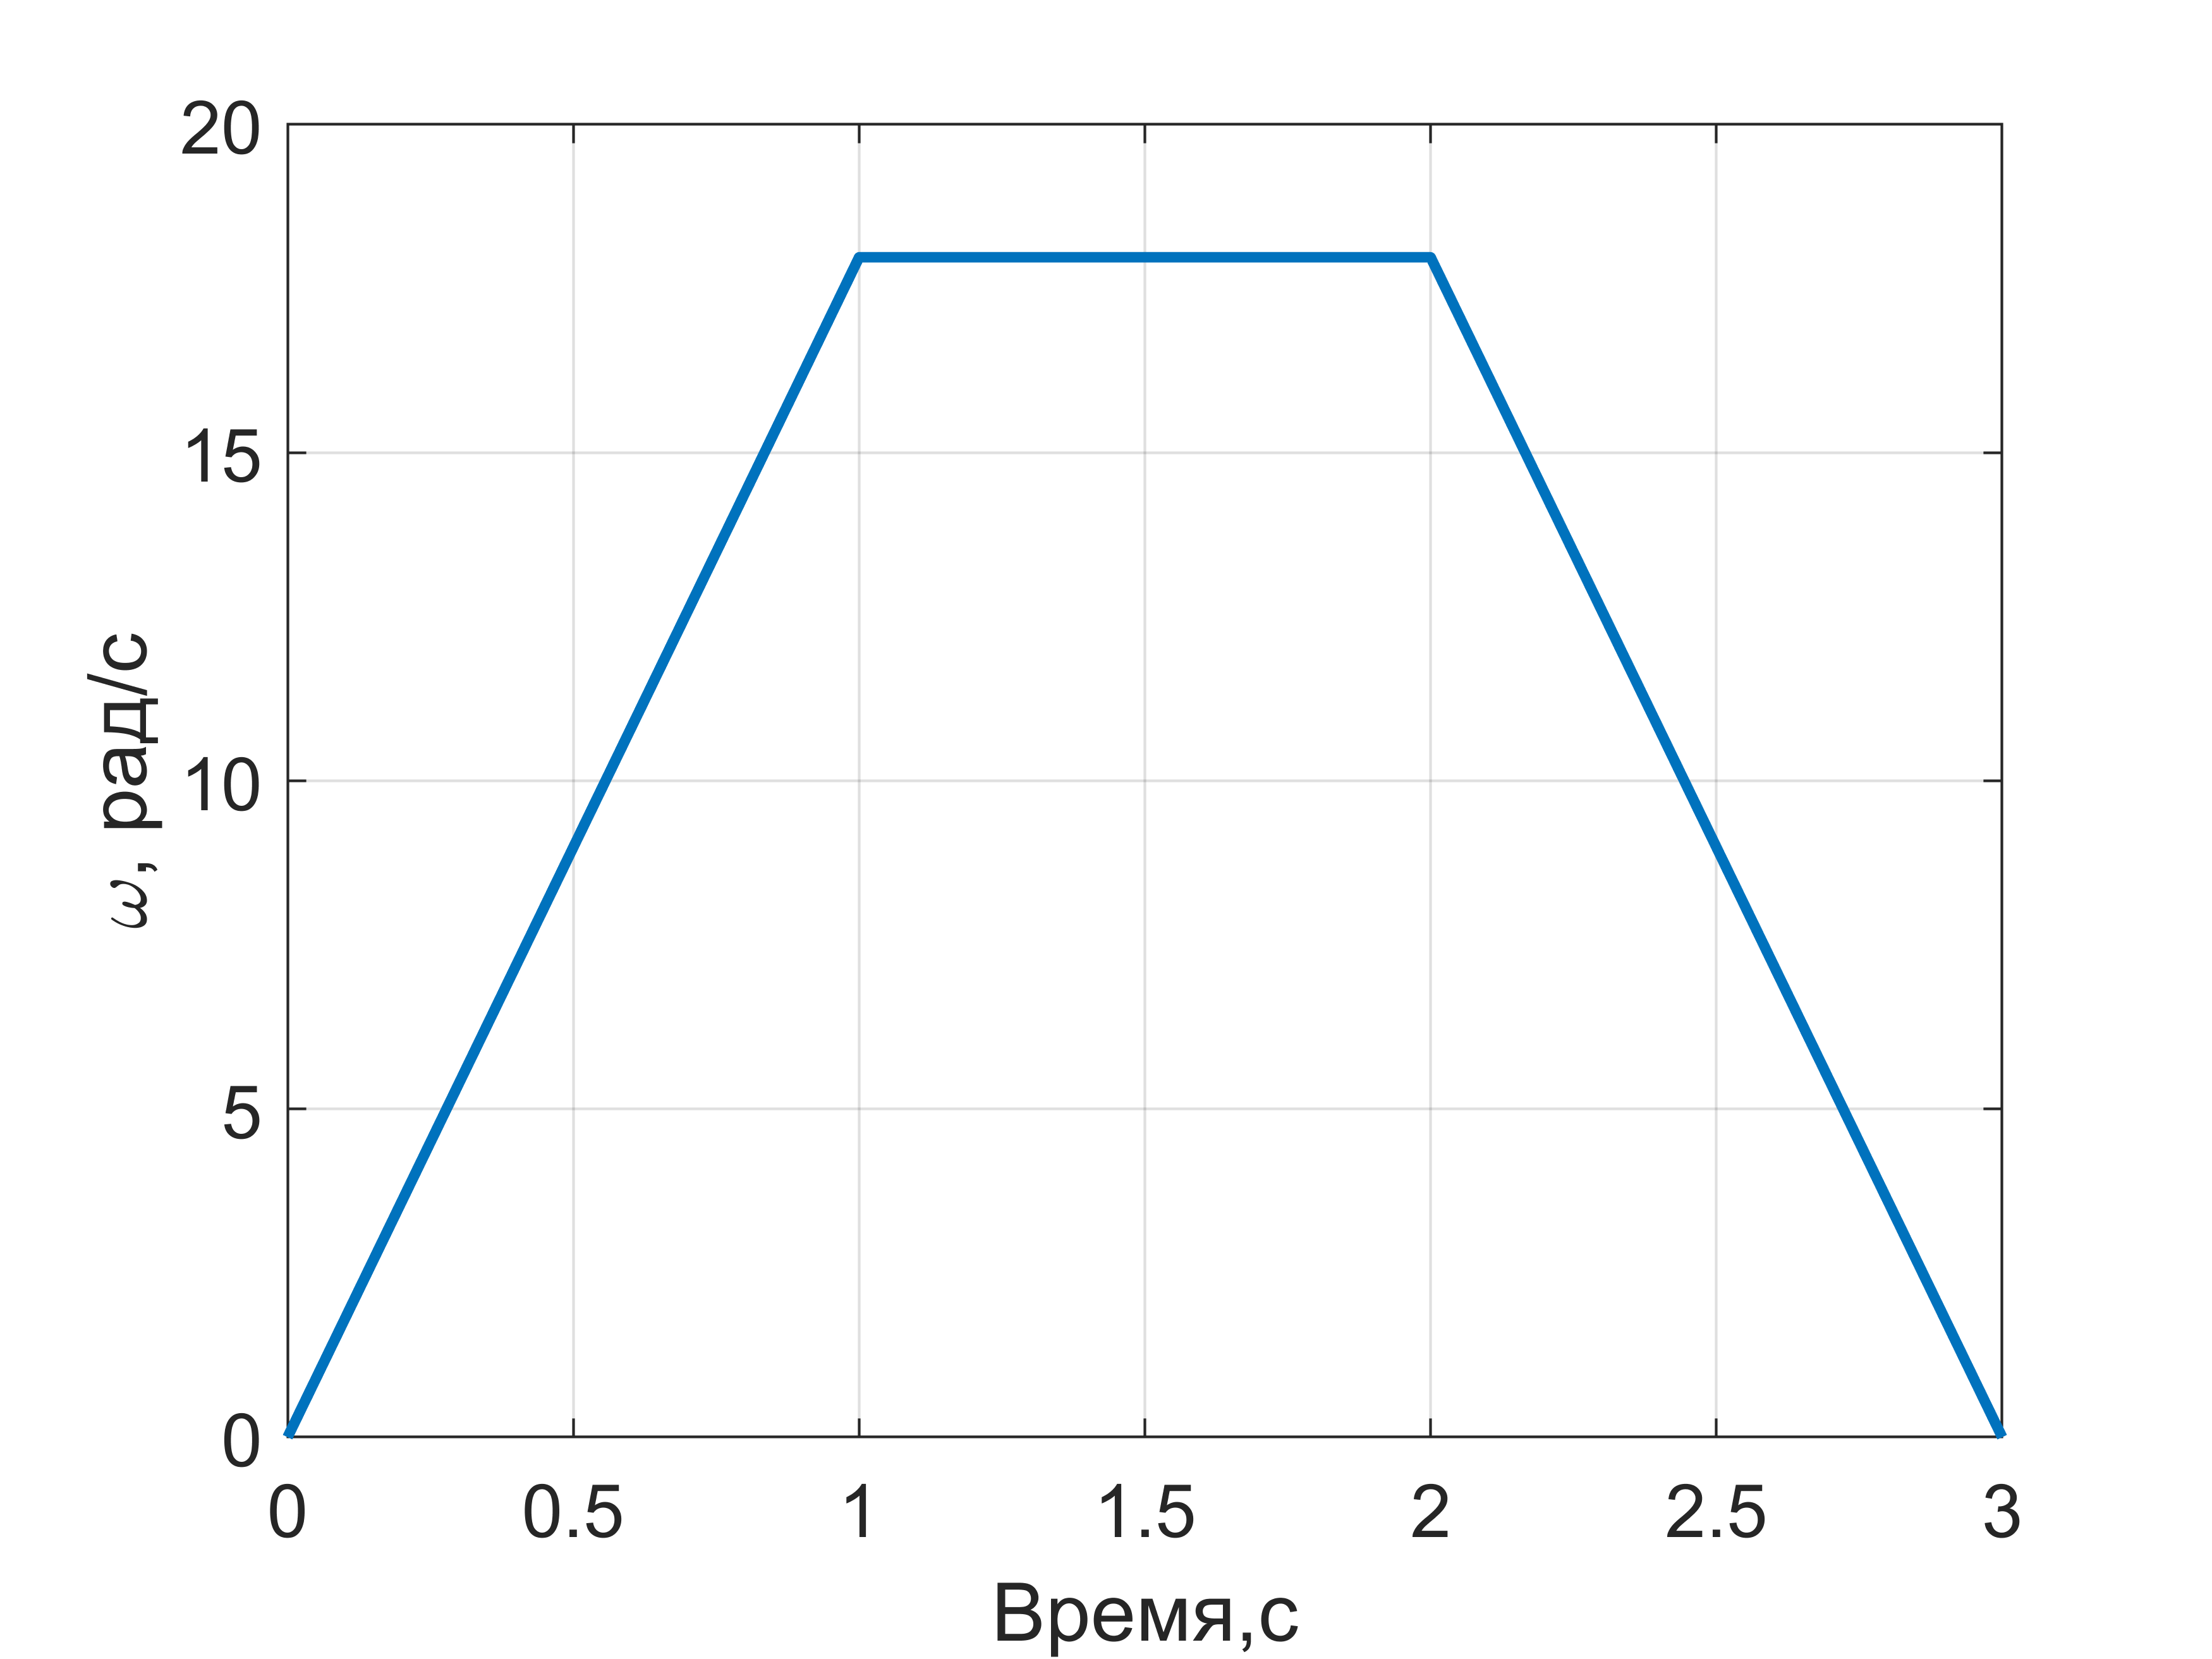
\includegraphics[scale=0.8]{matlab/img/flyweel_profile.png} 
	}
	\caption{Профиль разгона тестового маховика}
	\label{fig:flyweel_speed} 
\end{figure}



Скорость вращения определяется с помощью преобразователя угловых перемещений ЛИР-ДА190К. Угловая скорость определяется как отношение поворота маховика на угол $2\pi$ радиан к интервалу времени между двумя последовательными импульсами $t_{i+1}, t_i$ преобразователя: 

\begin{equation}
	\label{eq:flyweel_spd}
	\omega_i=\frac{2 \pi}{(t_{i+1}-t_i)}
\end{equation}

где \(i=1...5\) --- номер импульса.

Осциллограмма сигнала преобразователя представлена на рисунке ~\cref{fig:encoder}


\begin{figure}[!h] 
	\centerfloat{
		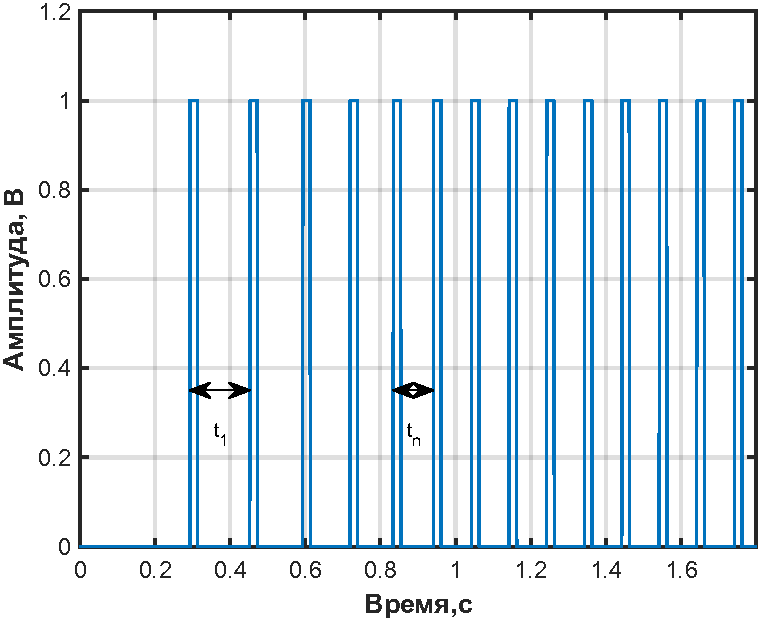
\includegraphics[scale=1]{matlab/img/encoder.pdf} 
	}
	\caption{Осциллограмма сигнала преобразователя угловых перемещений}
	\label{fig:encoder} 
\end{figure}

Угловое ускорение определяется так:

\begin{equation}
	\label{eq:flyweel_acc}
	\varepsilon = \frac{\omega_k-\omega_1}{t_k-t_1}
\end{equation}

где \(\omega_1, \omega_k\) --- начальная и конечная угловая скорость на участке разгона, \(t_1, t_k\) --- соответствующие моменты времени.

\subsection{Оценка бюджета погрешности}

Полный бюджет неопределённости формируется через разложение всех источников ошибок и последующее вычисление их вклада в итоговую величину измеряемого тестового момента. момент инерции маховика $J_m$ определяется один раз при сборке стенда на основе геометрических размеров и массы маховика. Измерения выполняются с использованием аттестованных средств измерений (штангенциркуля и весов), что гарантирует соответствие требованиям метрологического контроля. Погрешность измерения момента инерции составляет $\Delta J = 4.58 \cdot 10^{-7}\,\text{кг}\cdot\text{м}^2$ Подробный расчёт момента инерции приведён в приложении ~\ref{app:A}.

Для измерения углового ускорения маховика использовался преобразователь угловых перемещений, установленный на валу. преобразователь имеет паспортную погрешность $\Delta \phi = 10" = 4,85 \cdot 10^{-5} \text{~рад}$.

Маховику задается угловое ускорение $\alpha = 18.65 \,\text{рад/с}^{2}$. Измерение ускорения осуществляется косвенным методом --- через определение второй производной углового положения:

\begin{equation}
	\alpha = \frac{d^{2}\varphi}{dt^{2}}
\end{equation}

На практике вычисление производной производится численно по результатам дискретных измерений. При использовании центральной разности второго порядка для временного шага $\Delta t$ получаем:

\begin{equation}
	\alpha(t) \approx \frac{\varphi(t + \Delta t) - 2\varphi(t) + \varphi(t - \Delta t)}{\Delta t^{2}}
\end{equation}

Так как все измерения угла имеют погрешность $\Delta \phi$, она вносит вклад в неопределённость ускорения. При независимых ошибках трёх точек формулы для стандартной неопределённости ускорения принимает вид:

\begin{equation}
	u_{\alpha} = \frac{\sqrt{6}\,u_{\varphi}}{\Delta t^{2}}
\end{equation}

где \(u_\alpha\)"--- стандартная неопределённость измерения угла.

Паспортная величина $\pm10"$ задаётся как предел допускаемой абсолютной ошибки при равномерном распределении, то стандартная неопределённость:

\begin{equation}
	u_{\varphi} = \frac{\Delta \varphi}{\sqrt{3}} 
	\approx \frac{4.85 \cdot 10^{-5}}{\sqrt{3}} 
	\approx 2.8 \cdot 10^{-5} \,\text{рад}.
\end{equation}

Таким образом, итоговая погрешность ускорения зависит от выбранного временного интервала дискретизации $\Delta t$. В работе выбран шаг $\Delta t = \SI{0,02}{\second}$:

\begin{equation}
	u_{\alpha} = \frac{\sqrt{6} \cdot 2.8 \cdot 10^{-5}}{(0.02)^{2}}
	\approx 0.171 \,\text{рад/с}^{2}.
\end{equation}

Переходя от ускорения к моменту, отметим, что измеряемая величина задаётся произведением

\begin{equation}
	M = J \cdot \alpha
\end{equation}

а потому полная стандартная неопределённость момента, при независимости вкладов $J$ и $\alpha$, определяется законом распространения погрешностей:

\begin{equation}
	u_{M} = \sqrt{\left(\alpha \Delta J\right)^{2} + \left(J u_{\alpha}\right)^{2}}
\end{equation}

Подставляя числовые значения получим:

\begin{equation}
	u_{M} \approx \sqrt{(8.54 \times 10^{-6})^{2} + (4.61 \times 10^{-5})^{2}}
	\approx 4.7 \times 10^{-5} \,\text{Н·м}.
\end{equation}

Для полноты оценим и сам момент:

\begin{equation}
	M = J \alpha = 2.69 \times 10^{-4} \cdot 18.65 
	\approx 5.02 \times 10^{-3} \,\text{Н·м},
\end{equation}

а относительная неопределённость:

\begin{equation}
	\frac{u_{M}}{M} \approx 
	\frac{4.68 \times 10^{-5}}{5.02 \times 10^{-3}}
	\approx 0.93\% 
\end{equation}

Разработанный стенд прошёл метрологическую аттестацию в установленном порядке. 
Аттестация выполнена АО «НПО Техномаш» имени С.~А.~Афанасьева при поддержке 
Госкорпорации «Роскосмос». По результатам процедуры выдано свидетельство 
№~030-500/2024-61 (РОСС RU.0001.310066/2024), зарегистрированное в государственном 
реестре под номером ФР.1.28.2024.49055.

Методика измерения некомпенсированного возмущающего момента признана 
соответствующей требованиям ГОСТ~Р~8.563--2009. Диапазон измеряемых значений 
составляет от $10^{-3}$ до $1 \,\text{Н}\cdot\text{м}$.  

Таким образом, стенд обеспечивает требуемую точность измерений 
и может быть использован в качестве средства поверки и исследований 
оптико-механических систем. Сертификат аттестации представлен в приложении ~\cref{app:certificate}

	
\section{Измерение реактивного момента оптико-механической системы}

После установки изделия в изделиедержатель подвесная система переводится в состояние покоя. Для этого фиксируют платформу в исходном положении и ожидают затухания переходных процессов до уровня, при котором остаточные колебания не превышают допустимой амплитуды (менее 1 \% от рабочего сигнала гироскопа).

Задаётся эталонный момент с помощью тестового маховика. Скорость колебаний регистрируется гироскопом с частотой дискретизации $f_s=\SI{100}{\hertz}$. Для уменьшения случайных составляющих, измерения повторяются 10 раз. Усреднённый массив угловой скорости вычисляется по формуле:

\begin{equation}
	\label{eq:mean_spd}
	\overline{\omega_{i}}=\frac{1}{N}\sum_{j=1}^{N}\omega_{i}^{(j)}, \qquad N = 10.
\end{equation}

где \(\omega_{i}^j\) --- значение угловой скорости в $i-$ой точке при $j-$ом повторе.

Из усреднённого массива вычисляется угловое ускорение методом численного дифференцирования:

\begin{equation}
	\label{eq:mean_acc}
	\varepsilon_{i}
	= \frac{\overline{\omega}_{i+1}-\overline{\omega}_{i}}{\Delta t},
	\qquad
	\Delta t = \frac{1}{f_s}.
\end{equation}

На участке равноускоренного движения определяется среднее значение ускорения:


\begin{equation}
	\label{eq:acc}
	\varepsilon_m = \frac{1}{n}\sum_{i=1}^{n} \varepsilon_{i}
\end{equation}

где \(n\) --- число отсчётов на участке равномерного ускорения.

После задания эталонного момента выполняется измерение реактивного момента исследуемой ОМС. Привод изделия осуществляет поворот подвижной части на заданный угол. Под действием реактивного момента подвес совершает колебания, скорость которых  регистрирует гироскоп.

Данные обрабатываются аналогично: формируется усреднённый массив скорости колебаний:

\begin{equation}
	\label{eq:omega_op}
	\overline{\omega_{o_i}}
	= \frac{1}{N}\sum_{j=1}^{N} \omega_{o,i}^{(j)}
\end{equation}

После выполняется численное дифференцирование:

\begin{equation}
	\label{eq:epsilon_op}
	\varepsilon_{o_i}
	= \frac{\overline{\omega}_{o_i+1}
		- \overline{\omega}_{o,_i}}{\Delta t}\
\end{equation}

Среднее ускорение на равноускоренном участке находится как:

\begin{equation}
	\label{eq:epsilon_op_mean}
	\varepsilon_{o}
	= \frac{1}{n}\sum_{i=1}^{n} \varepsilon_{o_i}\,.
\end{equation}

Искомый остаточный реактивный момент рассчитывается через соотношение:

\begin{equation}
	\label{eq:Mom}
	M_o = M_m \cdot \frac{\varepsilon_o}{\varepsilon_m}
\end{equation}

Окончательное значение реактивного момента определяется как максимальное по модулю среди положительного и отрицательного экстремумов:

\begin{equation}
	\label{eq:Mom}
	M_{max} = max\{|M^+|, |M^-|\}
\end{equation}






\section*{Выводы по главе 3}

В данной главе разработан и создан испытательный стенд для измерения остаточных реактивных моментов оптико-механических систем.  
Построена теоретическая модель стенда в виде колебательного звена, что позволило определить требования к собственным частотам и декременту затухания подвесной системы. На основе анализа выбрана конструкция со струной в качестве упругого элемента, обеспечивающая малый уровень диссипативных потерь и одну степень свободы для исследуемого изделия.

Стенд оснащён волоконно-оптическим гироскопом для регистрации угловых колебаний и тестовым маховиком с известным моментом инерции для формирования эталонного воздействия. Разработана методика измерений, включающая юстировку подвесной системы, контроль климатических параметров и процедуры определения тестового момента. Проведена оценка бюджета погрешности, показавшая, что основными источниками неопределённости являются точность задания углового ускорения и погрешность измерения момента инерции маховика.

Созданный комплекс прошёл метрологическую аттестацию в установленном порядке, что подтверждает его пригодность для практического применения. Диапазон измеряемых значений составил от $10^{-3}$ до $1 \,\text{Н}\cdot\text{м}$ при относительной погрешности не более 1 \%. Это обеспечивает возможность достоверного определения остаточных реактивных моментов при испытаниях оптико-механических систем.

Таким образом, в работе сформирован базис для последующих экспериментальных исследований влияния реактивных моментов на смаз и качество изображений. 



\clearpage
\FloatBarrier